\documentclass{beamer}
\usepackage[en]{zafu}

% Charts & diagrams
\usepackage{pgfplots}
\usetikzlibrary{positioning, arrows.meta, shapes.geometric, calc, fit, shadows}
\pgfplotsset{compat=1.17}
\usepackage{booktabs}
\usepackage{array}
\usepackage{adjustbox}
\usepackage[style=numeric,backend=biber]{biblatex}
\addbibresource{daftar-pustaka.bib}

% Slightly smaller author & affiliation on title page
\setbeamerfont{author}{size=\small}
\setbeamerfont{institute}{size=\footnotesize}
\setbeamerfont{date}{size=\footnotesize}

% PDF metadata
\hypersetup{
  pdftitle={Kuantifikasi Unsur Tanah Vulkanik Menggunakan LIBS Berbasis Dekomposisi Spektral Multiunsur dengan CNN-Transformer},
  pdfauthor={Birrul Walidain},
  pdfsubject={LIBS; CNN-Transformer; Encoder-Decoder; Volcanic Soil},
  pdfkeywords={LIBS, CNN, Transformer, Encoder-Decoder, Volcanic Soil, Spectroscopy}
}
\pdfstringdefDisableCommands{%%
  \def\\{}%%
  \def\textsuperscript#1{#1}%%
}

% ----- Metadata -----
\title[Kuantifikasi Unsur LIBS]{%
  KUANTIFIKASI UNSUR TANAH VULKANIK MENGGUNAKAN LIBS \\
  BERBASIS DEKOMPOSISI SPEKTRAL MULTIUNSUR DENGAN \\
  CNN-TRANSFORMER }

\subtitle{Seminar Proposal Tesis}

\author[B.\,Walidain]{%
  Birrul Walidain\\[2pt]
  {\footnotesize NPM: 250820201100015}}

\institute{%
  \footnotesize
  Program Studi Magister Fisika\\
  Fakultas MIPA, Universitas Syiah Kuala\\[6pt]
  {\scriptsize
    Pembimbing I: Prof.\ Dr.\ Eng.\ Nasrullah, S.Si., M.T.\\
    Pembimbing II: Dr.\ Khairun Saddami, S.T.}}

\date{\today}

\titlegraphic{\includegraphics[width=0.16\textwidth]{src/logo-usk.png}}

\begin{document}

% Slide 1: Title
\maketitle

% Slide 2: Latar Belakang
\begin{frame}{Latar Belakang: Analisis Tanah \& Solusi LIBS-AI}
  \begin{figure}[H]
    \centering
    \includegraphics[height=0.99\textheight,keepaspectratio]{images/slide-2.png}
    % \caption{Alur perbandingan tantangan analisis tanah konvensional, solusi LIBS, dan potensi terapan kecerdasan buatan.}
  \end{figure}
\end{frame}

% Slide 3: Kompleksitas Spektrum Mineral Mezoued
\begin{frame}{Kompleksitas Spektrum Mineral Mezoued (2025)}
  \begin{figure}[H]
    \centering
    \includegraphics[height=0.9\textheight,keepaspectratio]{images/bab2/mezoued2025_fig1_mineral_spectra_complexity.png}
  \end{figure}
\end{frame}

% ==========================================
% Bagian A. Akar Masalah dan SOTA
% ==========================================
\section{Akar Masalah dan SOTA}

% Slide 4: Akar Masalah
\begin{frame}{Akar Masalah: Kompleksitas Spektrum LIBS}
  \begin{figure}[H]
    \centering
    \includegraphics[height=0.99\textheight,keepaspectratio]{images/libs_4panel.png}
  \end{figure}
\end{frame}

% Slide 5: Temuan Terdahulu (MERLIN)
\begin{frame}{Temuan Terdahulu: Model Transpor Radiatif MERLIN (Favre et al., 2025)}
  \begin{columns}[c]
    \begin{column}{0.48\textwidth}
      \centering
      \includegraphics[width=\textwidth,height=0.7\textheight,keepaspectratio]{images/bab2/favre2025_fig8_spectra_decomp.png}\\
      \vspace{0.4em}
      \fontsize{7pt}{8pt}\selectfont Dekomposisi spektrum emisi campuran
    \end{column}
    \begin{column}{0.48\textwidth}
      \centering
      \includegraphics[width=\textwidth,height=0.7\textheight,keepaspectratio]{images/bab2/favre2025_fig16_spectra_expvsmerlin.png}\\
      \vspace{0.4em}
      \fontsize{7pt}{8pt}\selectfont Spektrum eksperimen vs simulasi MERLIN
    \end{column}
  \end{columns}
\end{frame}

% Slide 6: Temuan Terdahulu (CNN)
\begin{frame}{Temuan Terdahulu: Spektroskopi LIBS Berbasis CNN (Favre et al., 2025)}
  \begin{columns}[c]
    \begin{column}{0.48\textwidth}
      \centering
      \includegraphics[width=\textwidth,height=0.7\textheight,keepaspectratio]{images/bab2/favre2025_table2.png}\\
      \vspace{0.4em}
      \fontsize{7pt}{8pt}\selectfont Tabel 2: Perbandingan parameter plasma dan fraksi mol
    \end{column}
    \begin{column}{0.48\textwidth}
      \centering
      \includegraphics[width=\textwidth,height=0.7\textheight,keepaspectratio]{images/bab2/favre2025_fig12_cnn_prediction.png}\\
      \vspace{0.4em}
      \fontsize{7pt}{8pt}\selectfont Spektrum prediksi CNN vs target fisis (truth)
    \end{column}
  \end{columns}
\end{frame}

% Slide 7: Temuan Terdahulu (Informer)
\begin{frame}{Temuan Terdahulu: Analisis Kualitatif Model Informer (Walidain et al., 2026)}
  \begin{columns}[c]
    \begin{column}{0.48\textwidth}
      \centering
      \includegraphics[width=\textwidth,height=0.7\textheight,keepaspectratio]{images/bab2/walidain2026_table2.png}\\
      \vspace{0.4em}
      \fontsize{7pt}{8pt}\selectfont Tabel 2: Presisi, recall, dan F1-score model Informer
    \end{column}
    \begin{column}{0.48\textwidth}
      \centering
      \includegraphics[width=\textwidth,height=0.7\textheight,keepaspectratio]{images/bab2/walidain2026_fig2_peakmatch.png}\\
      \vspace{0.4em}
      \fontsize{7pt}{8pt}\selectfont Pencocokan puncak emisi Mg dan Na hasil prediksi
    \end{column}
  \end{columns}
\end{frame}

% Slide 8: Temuan Terdahulu (Remote LIBS)
\begin{frame}{Temuan Terdahulu: Kuantifikasi Spektrum Remote LIBS (Liu et al., 2026)}
  \begin{columns}[c]
    \begin{column}{0.54\textwidth}
      \centering
      \includegraphics[width=\textwidth,height=0.7\textheight,keepaspectratio]{images/bab2/liu2026_fig5_spectrum.png}\\
      \vspace{0.4em}
      \fontsize{7pt}{8pt}\selectfont Spektrum observasi remote LIBS (10 meter)
    \end{column}
    \begin{column}{0.42\textwidth}
      \centering
      \includegraphics[width=\textwidth,height=0.7\textheight,keepaspectratio]{images/bab2/liu2026_fig4_scatter_p.png}\\
      \vspace{0.4em}
      \fontsize{7pt}{8pt}\selectfont Prediksi konsentrasi unsur P ($R^2 = 0.9924$)
    \end{column}
  \end{columns}
\end{frame}

% Slide 9: Solusi (Arsitektur Model)
\section{Solusi (Arsitektur Model)}

\begin{frame}{CNN-Transformer : Konse usulan penelitian ini}
  \begin{figure}[H]
    \centering
    \resizebox{!}{0.55\textheight}{
    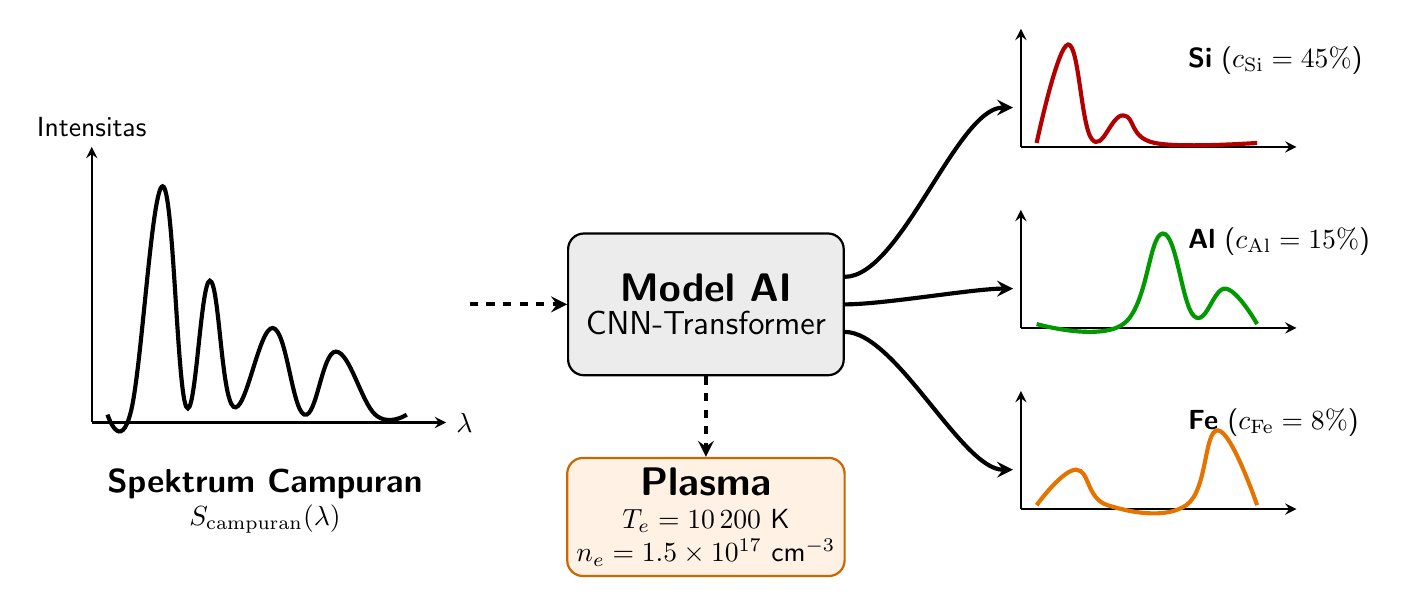
\begin{tikzpicture}[
        font=\sffamily,
        >=stealth,
        axis/.style={->, thick},
        curve/.style={line width=1.5pt},
        ai_box/.style={draw, thick, fill=gray!15, rounded corners=2mm, align=center, minimum width=3.5cm, minimum height=1.8cm},
        plasma_box/.style={draw=orange!80!black, thick, fill=orange!10, rounded corners=2mm, align=center, minimum width=3.5cm, minimum height=1.5cm}
    ]

    % ========================================================
    % 1. SPEKTRUM CAMPURAN (KIRI)
    % ========================================================
    \coordinate (O_mix) at (0,0);
    
    % Sumbu
    \draw[axis] (O_mix) -- ++(4.5,0) node[right] {$\lambda$};
    \draw[axis] (O_mix) -- ++(0,3.5) node[above] {Intensitas};
    
    % Kurva Spektrum Campuran (Superposisi)
    \draw[curve, black] plot[smooth, tension=0.7] coordinates {
        (0.2, 0.1) (0.5, 0.15) (0.9, 3.0) (1.2, 0.2) 
        (1.5, 1.8) (1.8, 0.2) (2.3, 1.2) (2.7, 0.1) 
        (3.1, 0.9) (3.6, 0.1) (4.0, 0.1)
    };
    
    % Label Nomenklatur
    \node[align=center] at (2.2, -1.0) {\large \textbf{Spektrum Campuran}\\ $S_{\mathrm{campuran}}(\lambda)$};

    % ========================================================
    % 2. BLOK MODEL AI & PARAMETER PLASMA (TENGAH)
    % ========================================================
    \node[ai_box] (ai) at (7.8, 1.5) {\Large \textbf{Model AI} \\ \large CNN-Transformer};
    
    \node[plasma_box] (plasma) at (7.8, -1.2) {\Large \textbf{Plasma} \\ \normalsize $T_e = 10\,200$ K \\ \normalsize $n_e = 1.5 \times 10^{17}$ cm$^{-3}$};

    % Panah Input
    \draw[->, dashed, line width=1.5pt] (4.8, 1.5) -- (ai.west);
    
    % Panah ke Parameter Plasma
    \draw[->, dashed, line width=1.5pt] (ai.south) -- (plasma.north);

    % ========================================================
    % 3. SPEKTRUM UNSUR TUNGGAL (KANAN)
    % ========================================================
    
    % -- A. Spektrum Si (Merah) --
    \coordinate (O_Si) at (11.8, 3.5);
    \draw[axis] (O_Si) -- ++(3.5,0);
    \draw[axis] (O_Si) -- ++(0,1.5);
    \draw[curve, red!70!black] plot[smooth, tension=0.7] coordinates {
        (12.0, 3.55) (12.4, 4.8) (12.7, 3.6) (13.1, 3.9) (13.5, 3.55) (14.8, 3.55)
    };
    \node[right] at (13.8, 4.6) {\textbf{Si} ($c_{\mathrm{Si}} = 45\%$)};

    % -- B. Spektrum Al (Hijau) --
    \coordinate (O_Al) at (11.8, 1.2);
    \draw[axis] (O_Al) -- ++(3.5,0);
    \draw[axis] (O_Al) -- ++(0,1.5);
    \draw[curve, green!60!black] plot[smooth, tension=0.7] coordinates {
        (12.0, 1.25) (13.1, 1.25) (13.6, 2.4) (14.0, 1.35) (14.4, 1.7) (14.8, 1.25)
    };
    \node[right] at (13.8, 2.3) {\textbf{Al} ($c_{\mathrm{Al}} = 15\%$)};

    % -- C. Spektrum Fe (Oranye) --
    \coordinate (O_Fe) at (11.8, -1.1);
    \draw[axis] (O_Fe) -- ++(3.5,0);
    \draw[axis] (O_Fe) -- ++(0,1.5);
    \draw[curve, orange!90!black] plot[smooth, tension=0.7] coordinates {
        (12.0, -1.05) (12.5, -0.6) (12.9, -1.05) (13.9, -1.05) (14.3, -0.1) (14.8, -1.05)
    };
    \node[right] at (13.8, 0) {\textbf{Fe} ($c_{\mathrm{Fe}} = 8\%$)};

    % Panah Dekomposisi dari Model ke Unsur
    \draw[->, line width=1.5pt] (ai.east) ++(0, 0.35) to[out=0, in=180, looseness=0.6] (11.7, 4.0);
    \draw[->, line width=1.5pt] (ai.east) to[out=0, in=180, looseness=0.6] (11.7, 1.7);
    \draw[->, line width=1.5pt] (ai.east) ++(0, -0.35) to[out=0, in=180, looseness=0.6] (11.7, -0.6);

    \end{tikzpicture}
    }
    % \caption{Makro arsitektur multi-stream dual-path yang memetakan spektrum campuran geologi tanah vulkanik.}
  \end{figure}
\end{frame}


% Slide 10: Research Questions \& Objectives
\begin{frame}{Research Questions \& Objectives}
  \begin{columns}[T,onlytextwidth]
    \begin{column}{0.48\textwidth}
      \textbf{Rumusan Masalah:}
      \vspace{0.5em}
      
      \centering
      \begin{tikzpicture}[
        node distance=0.35cm,
        rqbox/.style={rectangle, draw=maincolor, fill=maincolor!5, rounded corners=1mm,
          text width=4.8cm, align=center, font=\scriptsize\sffamily, minimum height=1.0cm, inner sep=1.5mm},
        arrow/.style={-{Stealth[length=2.5mm,width=2mm]}, thick, draw=maincolor!80}
      ]
        \node[rqbox] (rq1) {\textbf{RQ1}\\Bagaimana memodelkan hubungan antara \textbf{spektrum campuran} LIBS dengan \textbf{spektrum unsur tunggal}?};
        \node[rqbox, below=of rq1] (rq2) {\textbf{RQ2}\\Bagaimana merancang arsitektur \textbf{CNN-Transformer \textit{encoder-decoder}} untuk mengekstraksi fitur lokal \& global?};
        \node[rqbox, below=of rq2] (rq3) {\textbf{RQ3}\\Bagaimana kinerja model memprediksi \textbf{konsentrasi unsur \& parameter plasma} pada tanah vulkanik?};
        
        \draw[arrow] (rq1) -- (rq2);
        \draw[arrow] (rq2) -- (rq3);
      \end{tikzpicture}
    \end{column}

    \begin{column}{0.48\textwidth}
      \textbf{Tujuan Penelitian:}
      \vspace{0.5em}

      \centering
      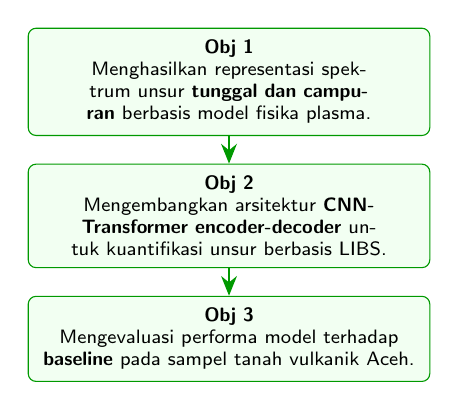
\begin{tikzpicture}[
        node distance=0.35cm,
        objbox/.style={rectangle, draw=green!60!black, fill=green!5, rounded corners=1mm,
          text width=4.8cm, align=center, font=\scriptsize\sffamily, minimum height=1.0cm, inner sep=1.5mm},
        arrow/.style={-{Stealth[length=2.5mm,width=2mm]}, thick, draw=green!60!black}
      ]
        \node[objbox] (obj1) {\textbf{Obj 1}\\Menghasilkan representasi spektrum unsur \textbf{tunggal dan campuran} berbasis model fisika plasma.};
        \node[objbox, below=of obj1] (obj2) {\textbf{Obj 2}\\Mengembangkan arsitektur \textbf{CNN-Transformer \textit{encoder-decoder}} untuk kuantifikasi unsur berbasis LIBS.};
        \node[objbox, below=of obj2] (obj3) {\textbf{Obj 3}\\Mengevaluasi performa model terhadap \textbf{\textit{baseline}} pada sampel tanah vulkanik Aceh.};
        
        \draw[arrow] (obj1) -- (obj2);
        \draw[arrow] (obj2) -- (obj3);
      \end{tikzpicture}
    \end{column}
  \end{columns}
\end{frame}


% Slide 11: Visualisasi Konsep Tokenisasi
\begin{frame}{Visualisasi Konsep Tokenisasi: Sliding Window Spektroskopi}
  \begin{figure}[H]
    \centering
    \includegraphics[width=0.92\textwidth,height=0.72\textheight,keepaspectratio]{images/spectral_zoom_cnn.png}
    \caption{Visualisasi pemotongan spektrum campuran (window 320--330 nm) yang dikirim ke Tokenizer CNN 1D.}
    \label{fig:spectral_zoom_cnn}
  \end{figure}
\end{frame}

% Slide 12: Visualisasi Input Model
\begin{frame}{Visualisasi Input Model: Campuran (Encoder) vs Unsur Tunggal (Decoder)}
  \begin{columns}[c]
    \begin{column}{0.54\textwidth}
      \begin{figure}[H]
        \centering
        \includegraphics[width=\textwidth,keepaspectratio]{images/enc_dec_inputs.png}
        \caption{Spektrum 10 nm terfokus (320--330 nm) hasil simulasi plasma 7000 K.}
        \label{fig:enc_dec_inputs}
      \end{figure}
    \end{column}
    \begin{column}{0.44\textwidth}
      \centering
      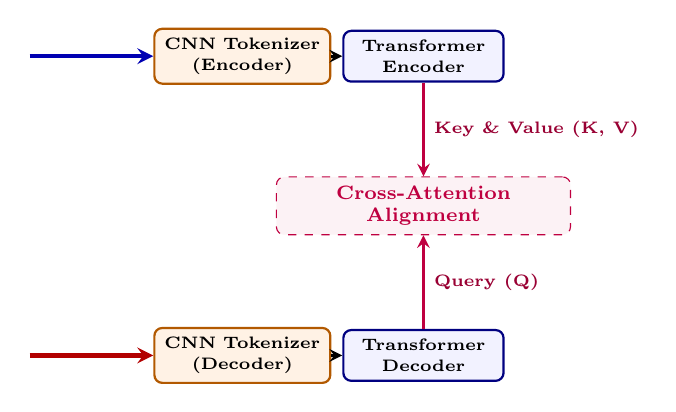
\begin{tikzpicture}[
          font=\sffamily,
          >=stealth,
          box/.style={draw, thick, rounded corners=1mm, align=center, text width=2.0cm, minimum height=0.6cm, font=\fontsize{6.5pt}{7.5pt}\selectfont},
          cnn_box/.style={box, fill=orange!10, draw=orange!70!black},
          model_box/.style={box, fill=blue!5, draw=blue!50!black, text width=1.8cm},
          arrow/.style={-stealth, line width=1.0pt}
      ]
          % Jalur Campuran (Encoder Path) - Panah dari plot atas di kiri
          \node[cnn_box] (cnn_enc) at (-2.2, 4.3) {\textbf{CNN Tokenizer}\\\textbf{(Encoder)}};
          \node[model_box] (enc) at (0.1, 4.3) {\textbf{Transformer}\\\textbf{Encoder}};
          
          \draw[arrow, draw=blue!70!black, line width=1.5pt] (-4.9, 4.3) -- (cnn_enc.west);
          \draw[arrow] (cnn_enc) -- (enc);
          
          % Interaksi Cross-Attention di tengah
          \node[draw, dashed, purple, rounded corners=1mm, fill=purple!5, font=\fontsize{7pt}{8pt}\selectfont\bfseries, align=center, text width=3.5cm] (ca) at (0.1, 2.4) {Cross-Attention Alignment};
          \draw[arrow, ->, draw=purple] (enc.south) -- node[right, font=\fontsize{6.5pt}{7.5pt}\selectfont\bfseries, color=purple!80!black] {Key \& Value (K, V)} (ca.north);
          
          % Jalur Unsur Tunggal (Decoder Path) - Panah dari plot bawah di kiri
          \node[cnn_box] (cnn_dec) at (-2.2, 0.5) {\textbf{CNN Tokenizer}\\\textbf{(Decoder)}};
          \node[model_box] (dec) at (0.1, 0.5) {\textbf{Transformer}\\\textbf{Decoder}};
          
          \draw[arrow, draw=red!70!black, line width=1.5pt] (-4.9, 0.5) -- (cnn_dec.west);
          \draw[arrow] (cnn_dec) -- (dec);
          \draw[arrow, ->, draw=purple] (dec.north) -- node[right, font=\fontsize{6.5pt}{7.5pt}\selectfont\bfseries, color=purple!80!black] {Query (Q)} (ca.south);
      \end{tikzpicture}
    \end{column}
  \end{columns}
\end{frame}

% Slide 13: Mekanisme Utama (Cross-Attention)
\begin{frame}{Mekanisme Utama: Cross-Attention Decomposer}
  \vspace{-0.5em}
  \begin{figure}[H]
    \centering
    \begin{adjustbox}{max width=\textwidth, max totalheight=0.80\textheight, keepaspectratio, center}
    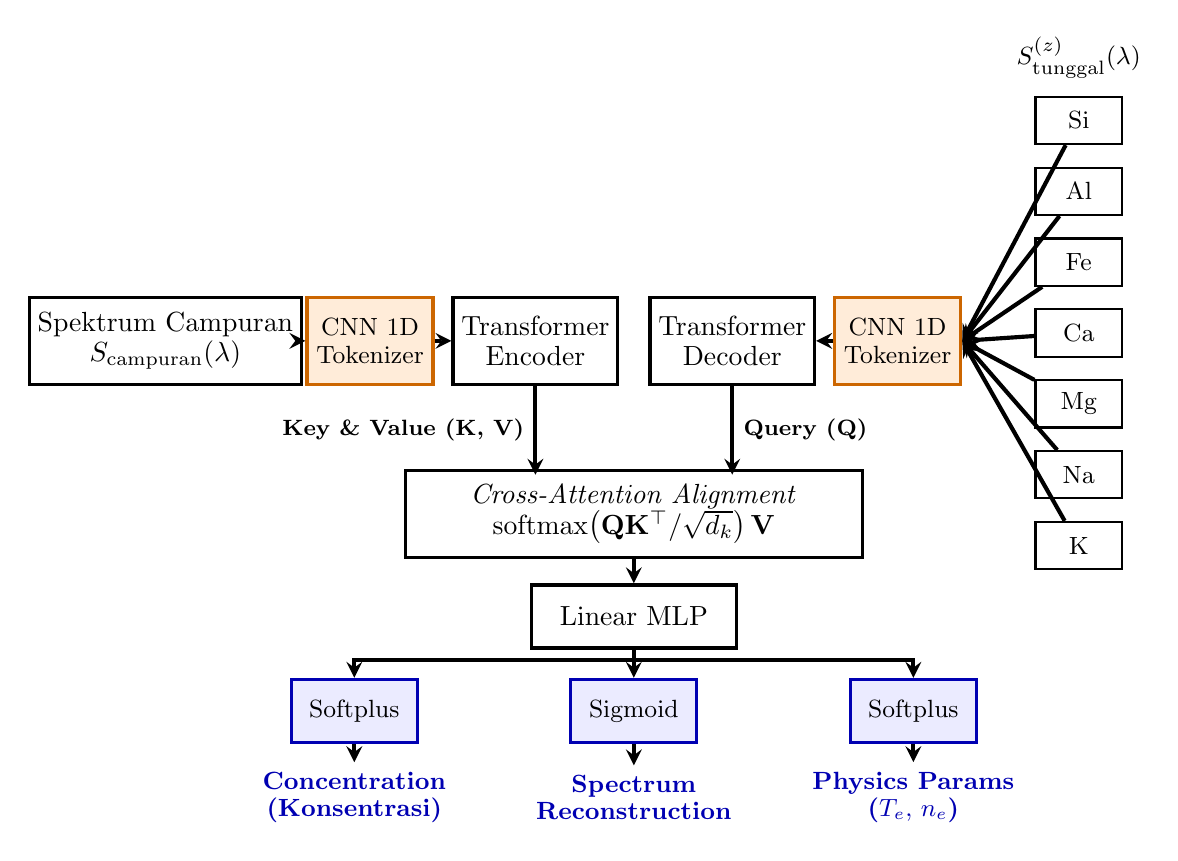
\begin{tikzpicture}[font=\normalsize,
      elem/.style={draw, thick, minimum width=1.1cm, minimum height=0.6cm, inner sep=2pt, font=\fontsize{9pt}{10pt}\selectfont},
      blok/.style={draw, very thick, align=center, minimum height=1.1cm, inner sep=3pt, font=\fontsize{10pt}{11pt}\selectfont},
      cnn/.style={draw, very thick, fill=orange!15, draw=orange!80!black, align=center, minimum height=1.1cm, inner sep=3pt, font=\fontsize{9pt}{10pt}\selectfont},
      outblok/.style={draw, very thick, fill=blue!8, draw=blue!70!black, align=center, minimum height=1.0cm, inner sep=3pt, font=\fontsize{9pt}{10pt}\selectfont},
      panah/.style={-stealth, line width=1.5pt}]
      
      % kiri: spektrum campuran
      \node[blok, minimum width=2.8cm] (mix) at (0.0,2.8) {Spektrum Campuran\\ $S_{\mathrm{campuran}}(\lambda)$};
      % CNN Tokenizer Kiri
      \node[cnn, minimum width=1.6cm] (cnn_enc) at (2.6,2.8) {CNN 1D\\ Tokenizer};
      % Encoder
      \node[blok, minimum width=1.8cm] (enc) at (4.7,2.8) {Transformer\\ Encoder};
      
      \draw[panah] (mix) -- (cnn_enc);
      \draw[panah] (cnn_enc) -- (enc);
      
      % kanan: tujuh spektrum unsur tunggal
      \node[elem] (e1) at (11.6,5.6) {Si};
      \node[elem] (e2) at (11.6,4.7) {Al};
      \node[elem] (e3) at (11.6,3.8) {Fe};
      \node[elem] (e4) at (11.6,2.9) {Ca};
      \node[elem] (e5) at (11.6,2.0) {Mg};
      \node[elem] (e6) at (11.6,1.1) {Na};
      \node[elem] (e7) at (11.6,0.2) {K};
      \node[align=center, font=\fontsize{9.5pt}{10.5pt}\selectfont\bfseries] at (11.6,6.4) {$S_{\mathrm{tunggal}}^{(z)}(\lambda)$};
      
      % CNN Tokenizer Kanan
      \node[cnn, minimum width=1.6cm] (cnn_dec) at (9.3,2.8) {CNN 1D\\ Tokenizer};
      % Decoder
      \node[blok, minimum width=1.8cm] (dec) at (7.2,2.8) {Transformer\\ Decoder};
      
      \foreach \i in {1,...,7} \draw[panah] (e\i) -- (cnn_dec.east);
      \draw[panah] (cnn_dec) -- (dec);
      
      % cross-attention (tengah bawah)
      \node[blok, minimum width=5.8cm] (ca) at (5.95,0.6)
        {\textit{Cross-Attention Alignment}\\ $\mathrm{softmax}\!\left(\mathbf{Q}\mathbf{K}^{\top}/\sqrt{d_k}\right)\mathbf{V}$};
        
      \draw[panah] (enc.south) -- node[left, font=\fontsize{8.5pt}{9.5pt}\selectfont\bfseries] {Key \& Value (K, V)} (4.7,1.1);
      \draw[panah] (dec.south) -- node[right, font=\fontsize{8.5pt}{9.5pt}\selectfont\bfseries] {Query (Q)} (7.2,1.1);
      
      % Linear MLP
      \node[blok, minimum width=2.6cm, minimum height=0.8cm] (mlp) at (5.95,-0.7) {Linear MLP};
      \draw[panah] (ca.south) -- (mlp);
      
      % Kiri: Softplus -> Concentration
      \node[outblok, minimum width=1.6cm, minimum height=0.8cm] (act_conc) at (2.4,-1.9) {Softplus};
      \node[align=center, font=\fontsize{9pt}{10pt}\selectfont\bfseries, color=blue!70!black] (out_conc) at (2.4,-3.0) {Concentration\\ (Konsentrasi)};
      \draw[panah] (mlp.south) -- (5.95,-1.25) -- (2.4,-1.25) -- (act_conc.north);
      \draw[panah] (act_conc) -- (out_conc);
      
      % Tengah: Sigmoid -> Spectrum Reconstruction
      \node[outblok, minimum width=1.6cm, minimum height=0.8cm] (act_spec) at (5.95,-1.9) {Sigmoid};
      \node[align=center, font=\fontsize{9pt}{10pt}\selectfont\bfseries, color=blue!70!black] (out_spec) at (5.95,-3.0) {Spectrum\\ Reconstruction};
      \draw[panah] (mlp.south) -- (act_spec.north);
      \draw[panah] (act_spec) -- (out_spec);
      
      % Kanan: Softplus -> Physics Params
      \node[outblok, minimum width=1.6cm, minimum height=0.8cm] (act_phys) at (9.5,-1.9) {Softplus};
      \node[align=center, font=\fontsize{9pt}{10pt}\selectfont\bfseries, color=blue!70!black] (out_phys) at (9.5,-3.0) {Physics Params\\ ($T_e,\, n_e$)};
      \draw[panah] (mlp.south) -- (5.95,-1.25) -- (9.5,-1.25) -- (act_phys.north);
      \draw[panah] (act_phys) -- (out_phys);
    \end{tikzpicture}
    \end{adjustbox}
  \end{figure}
\end{frame}

% Slide 14: Validasi Luaran \& Dekomposisi Model
\begin{frame}{Validasi Luaran \& Dekomposisi Model}
  \begin{columns}[c]
    \begin{column}{0.48\textwidth}
      \begin{figure}[H]
        \centering
        \includegraphics[height=0.9\textheight,keepaspectratio]{images/model_outputs.png}
        \vspace{-0.4em}
        \caption{\fontsize{6.5pt}{7.5pt}\selectfont Hasil dekomposisi fisis model: (A) Rekonstruksi spektrum Ca \& Fe, (B) Prediksi konsentrasi.}
        \label{fig:model_outputs}
      \end{figure}
    \end{column}
    \begin{column}{0.48\textwidth}
      \centering
      {\normalsize\color{orange!80!black}\textbf{C. Estimasi Parameter Plasma}}
      
      \vspace{0.4em}
      \resizebox{\textwidth}{!}{
        \begin{tabular}{lccc}
          \hline
          \textbf{Parameter} & \textbf{Ground Truth} & \textbf{Prediksi Model} & \textbf{Akurasi} \\
          \hline
          Suhu ($T_e$) & 7000 K & 6982 K & 99.74 \% \\
          Kerapatan ($n_e$) & $1.50 \times 10^{17}\text{ cm}^{-3}$ & $1.49 \times 10^{17}\text{ cm}^{-3}$ & 99.33 \% \\
          \hline
        \end{tabular}
      }
      
      \vspace{1.0em}
      \flushleft
      {\normalsize\color{orange!80!black}\textbf{Karakteristik Dekomposisi:}}
      \vspace{0.2em}
      \fontsize{7.0pt}{9.0pt}\selectfont
      \begin{itemize}
        \item \textbf{Resolusi Multi-Unsur:} Model memisahkan kontribusi emisi murni Ca dan Fe dari campuran tumpang tindih secara simultan.
        \item \textbf{Akurasi Tinggi:} Konsentrasi diestimasi dengan tingkat kesesuaian sangat tinggi terhadap ground truth.
      \end{itemize}
    \end{column}
  \end{columns}
\end{frame}


% Slide 15: Adaptasi Domain (GRL)
\begin{frame}{Adaptasi Domain: Gradient Reversal Layer (GRL)}
  \vspace{-0.3em}
  \begin{figure}[H]
    \centering
    \begin{adjustbox}{max width=\textwidth, max totalheight=0.74\textheight, keepaspectratio, center}
    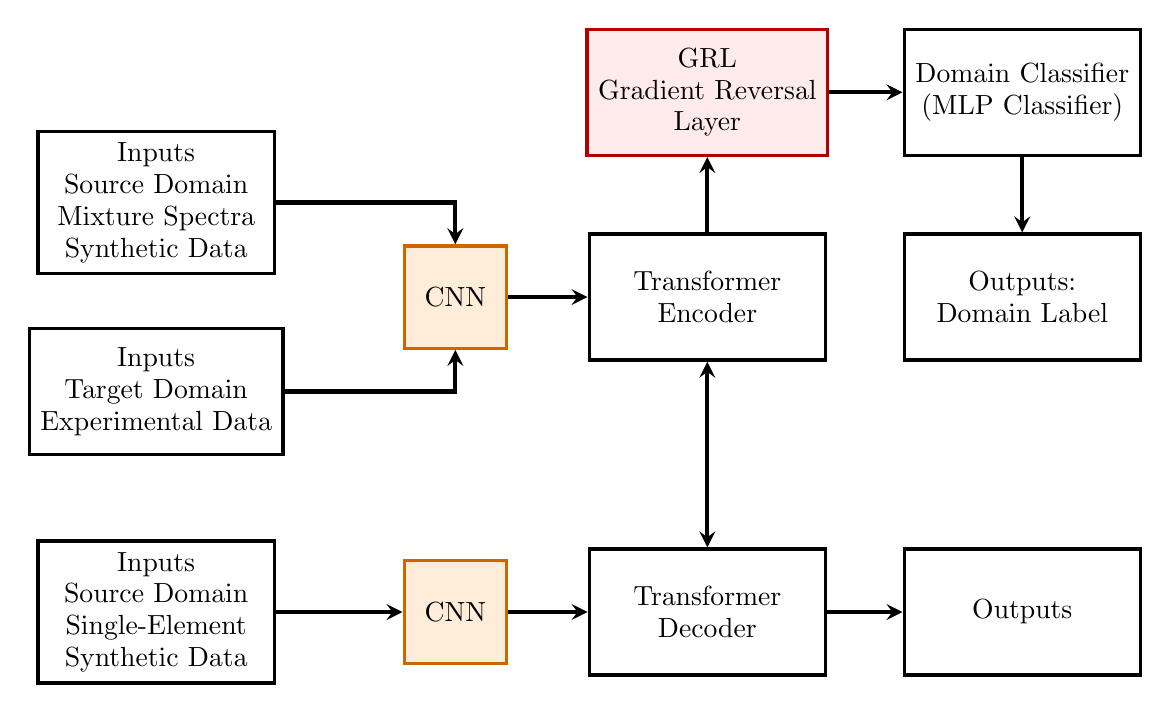
\begin{tikzpicture}[font=\normalsize,
      blok/.style={draw, very thick, align=center, minimum width=3.0cm, minimum height=1.6cm, inner sep=4pt, font=\fontsize{10pt}{11.5pt}\selectfont},
      cnnblok/.style={draw, very thick, fill=orange!15, draw=orange!80!black, align=center, minimum width=1.3cm, minimum height=1.3cm, inner sep=3pt, font=\fontsize{10pt}{11pt}\selectfont},
      grlblok/.style={draw=red!70!black, very thick, fill=red!8, align=center, minimum width=3.0cm, minimum height=1.6cm, inner sep=4pt, font=\fontsize{10pt}{11.5pt}\selectfont},
      panah/.style={-stealth, line width=1.5pt},
      dpanah/.style={stealth-stealth, line width=1.5pt}
    ]

    % ─── Input nodes (kolom kiri) ───────────────────────────────
    \node[blok] (mix)    at (0,  3.2) {Inputs\\ Source Domain\\ Mixture Spectra\\ Synthetic Data};
    \node[blok] (target) at (0,  0.8) {Inputs\\ Target Domain\\ Experimental Data};
    \node[blok] (single) at (0, -2.0) {Inputs\\ Source Domain\\ Single-Element\\ Synthetic Data};

    % ─── CNN blocks ──────────────────────────────────────────────
    \node[cnnblok] (cnn_enc) at (3.8, 2.0) {CNN};
    \node[cnnblok] (cnn_dec) at (3.8, -2.0) {CNN};

    % ─── Transformer Encoder & Decoder ───────────────────────────
    \node[blok] (enc) at (7.0, 2.0) {Transformer\\ Encoder};
    \node[blok] (dec) at (7.0, -2.0) {Transformer\\ Decoder};

    % ─── GRL (atas Encoder) ──────────────────────────────────────
    \node[grlblok] (grl) at (7.0, 4.6) {GRL\\ Gradient Reversal\\ Layer};

    % ─── Domain Classifier & Label ───────────────────────────────
    \node[blok] (dc) at (11.0, 4.6) {Domain Classifier\\ (MLP Classifier)};
    \node[blok] (dl) at (11.0, 2.0) {Outputs:\\ Domain Label};

    % ─── Outputs (bottom right) ──────────────────────────────────
    \node[blok] (out) at (11.0, -2.0) {Outputs};

    % ─── Arrows ──────────────────────────────────────────────────
    % Inputs → CNN shared
    \draw[panah] (mix.east)    -| (cnn_enc.north);
    \draw[panah] (target.east) -| (cnn_enc.south);

    % CNN → Encoder
    \draw[panah] (cnn_enc) -- (enc);

    % Encoder → GRL (vertical up)
    \draw[panah] (enc.north) -- (grl.south);

    % GRL → Domain Classifier (horizontal)
    \draw[panah] (grl) -- (dc);

    % Domain Classifier → Domain Label (vertical down)
    \draw[panah] (dc.south) -- (dl.north);

    % Encoder ↔ Decoder (double-headed, cross-attention)
    \draw[dpanah] (enc.south) -- (dec.north);

    % Bottom row: Single-Element path
    \draw[panah] (single)   -- (cnn_dec);
    \draw[panah] (cnn_dec)  -- (dec);
    \draw[panah] (dec)      -- (out);

    \end{tikzpicture}
    \end{adjustbox}
  \end{figure}
  \vspace{-0.2em}
  \centering
  \small $\mathcal{L}_{\mathrm{total}} = \mathcal{L}_{\mathrm{prediksi}} - \lambda\,\mathcal{L}_{\mathrm{domain}}$
\end{frame}

% ==========================================
% Bagian C. Protokol Penelitian
% ==========================================
\section{Protokol Penelitian}
% Slide 16: Protokol Penelitian \& Alur Kerja
\begin{frame}{Protokol Penelitian \& Alur Kerja}
\vspace{-0.5em}
\begin{center}
\begin{adjustbox}{max width=\textwidth, max totalheight=0.82\textheight, keepaspectratio}
\begin{tikzpicture}[font=\sffamily]

  % Definisi Gaya Teks
  \tikzset{
    header text/.style={white, anchor=north west, text width=5.0cm, font=\bfseries\fontsize{8pt}{9pt}\selectfont}
  }

  % ==========================================
  % TAHAP I: KIRI ATAS (Simulasi)
  % ==========================================
  \begin{scope}
    \clip[rounded corners=3pt] (-6.1cm,0.4cm) rectangle (-0.9cm,3.2cm);
    \fill[blue!10] (-6.1cm,0.4cm) rectangle (-0.9cm,3.2cm);
    \fill[blue!80!black] (-6.1cm,2.65cm) rectangle (-0.9cm,3.2cm);
  \end{scope}
  \draw[blue!80!black, line width=1.2pt, rounded corners=3pt] (-6.1cm,0.4cm) rectangle (-0.9cm,3.2cm);
  
  \node[header text] at (-6.02cm,3.08cm) {Tahap I — Simulasi};
  \node[anchor=south west, inner sep=0] at (-6.05cm, 0.45cm) {
    \includegraphics[width=5.1cm, height=2.15cm, keepaspectratio=false]{images/tahap1_sim_spectra.png}
  };

  % ==========================================
  % TAHAP II: KANAN ATAS (Akuisisi)
  % ==========================================
  \begin{scope}
    \clip[rounded corners=3pt] (0.9cm,0.4cm) rectangle (6.1cm,3.2cm);
    \fill[teal!10] (0.9cm,0.4cm) rectangle (6.1cm,3.2cm);
    \fill[teal!80!black] (0.9cm,2.65cm) rectangle (6.1cm,3.2cm);
  \end{scope}
  \draw[teal!80!black, line width=1.2pt, rounded corners=3pt] (0.9cm,0.4cm) rectangle (6.1cm,3.2cm);
  
  \node[header text] at (0.98cm,3.08cm) {Tahap II — Akuisisi};
  \node[anchor=south west, inner sep=0] at (0.95cm, 0.45cm) {
    \includegraphics[width=5.1cm, height=2.15cm, keepaspectratio=false]{images/tahap2_exp_spectra.png}
  };

  % ==========================================
  % TAHAP III: KANAN BAWAH (Pelatihan)
  % ==========================================
  \begin{scope}
    \clip[rounded corners=3pt] (0.9cm,-3.2cm) rectangle (6.1cm,-0.4cm);
    \fill[purple!10] (0.9cm,-3.2cm) rectangle (6.1cm,-0.4cm);
    \fill[purple!80!black] (0.9cm,-0.95cm) rectangle (6.1cm,-0.4cm);
  \end{scope}
  \draw[purple!80!black, line width=1.2pt, rounded corners=3pt] (0.9cm,-3.2cm) rectangle (6.1cm,-0.4cm);
  
  \node[header text] at (0.98cm,-0.52cm) {Tahap III — Pelatihan};
  \node[anchor=south west, inner sep=0] at (0.95cm, -3.15cm) {
    \includegraphics[width=5.1cm, height=2.15cm, keepaspectratio=false]{images/tahap3_loss_curve.png}
  };

  % ==========================================
  % TAHAP IV: KIRI BAWAH (Evaluasi)
  % ==========================================
  \begin{scope}
    \clip[rounded corners=3pt] (-6.1cm,-3.2cm) rectangle (-0.9cm,-0.4cm);
    \fill[red!10] (-6.1cm,-3.2cm) rectangle (-0.9cm,-0.4cm);
    \fill[red!80!black] (-6.1cm,-0.95cm) rectangle (-0.9cm,-0.4cm);
  \end{scope}
  \draw[red!80!black, line width=1.2pt, rounded corners=3pt] (-6.1cm,-3.2cm) rectangle (-0.9cm,-0.4cm);
  
  \node[header text] at (-6.02cm,-0.52cm) {Tahap IV — Evaluasi};
  \node[anchor=south west, inner sep=0] at (-6.05cm, -3.15cm) {
    \includegraphics[width=5.1cm, height=2.15cm, keepaspectratio=false]{images/tahap4_eval_te.png}
  };

  % ==========================================
  % PANAH ALUR & LUARAN TAHAPAN (Tepi & Luar Kotak)
  % ==========================================
  \tikzset{
    arrow flow/.style={-stealth, gray!80, line width=2.0pt, opacity=0.95},
    label flow/.style={gray!90, font=\fontsize{6.5pt}{7.5pt}\selectfont\bfseries, align=center, inner sep=2pt}
  }

  % T1 -> T2: Horizontal Tengah Atas (Dataset Sintetis di atas panah)
  \draw[arrow flow] (-0.9cm, 1.8cm) -- (0.9cm, 1.8cm) 
    node[midway, above=1pt, label flow] {Dataset\\ Sintetis};

  % T2 -> T3: Siku Kanan Luar (Dataset Penuh di sebelah kanan panah vertikal luar)
  \draw[arrow flow] (6.1cm, 1.8cm) -- (6.5cm, 1.8cm) -- (6.5cm, -1.8cm) -- (6.1cm, -1.8cm);
  \node[label flow, anchor=west] at (6.6cm, 0) {Dataset\\ Penuh};

  % T3 -> T4: Horizontal Tengah Bawah (Model Konvergen di atas panah)
  \draw[arrow flow] (0.9cm, -1.8cm) -- (-0.9cm, -1.8cm)
    node[midway, above=1pt, label flow] {Model\\ Konvergen};

\end{tikzpicture}
\end{adjustbox}
\end{center}
\end{frame}

% Slide 17: Prosedur: Tahap I — Simulasi
\begin{frame}{Prosedur: Tahap I — Simulasi}
  \begin{center}
    \begin{adjustbox}{max width=\textwidth, max totalheight=0.85\textheight, keepaspectratio}
      \begin{tikzpicture}[font=\sffamily]
        % Garis memotong di tengah (silang)
        \draw[gray!30, line width=1.0pt] (-5.8, 0) -- (5.8, 0);
        \draw[gray!30, line width=1.0pt] (0, -3.2) -- (0, 3.2);

        % ==========================================
        % KUADRAN I: KIRI ATAS (Parameter & NIST ASD)
        % ==========================================
        \node[anchor=north west, font=\fontsize{9.5pt}{11pt}\selectfont\bfseries, color=blue!85!black] at (-5.7, 3.0) {1. Parameter Fisis \& NIST ASD};
        \node[anchor=north east] at (-0.3, 2.6) {
          \fontsize{6.5pt}{8.0pt}\selectfont
          \setlength{\tabcolsep}{4.5pt}
          \renewcommand{\arraystretch}{1.2}
          \begin{tabular}{ccccc}
            \toprule
            \textbf{Unsur} & \textbf{Spesies} & \textbf{$\lambda$ (nm)} & \textbf{Energi ($E_i - E_k$)} & \textbf{$A_{ki}$ (s$^{-1}$)} \\
            \midrule
            Si & Si I & 288,16 & 0,78 -- 5,08 eV & 1,89e8 \\
            Al & Al I & 309,27 & 0,02 -- 4,02 eV & 7,37e7 \\
            Fe & Fe I & 373,49 & 0,05 -- 3,37 eV & 1,62e8 \\
            Ca & Ca II & 393,37 & 0,00 -- 3,15 eV & 1,47e8 \\
            Mg & Mg I & 285,21 & 0,00 -- 4,35 eV & 2,91e8 \\
            \bottomrule
          \end{tabular}
        };

        % ==========================================
        % KUADRAN II: KANAN ATAS (Saha-Boltzmann)
        % ==========================================
        \node[anchor=north west, font=\fontsize{9.5pt}{11pt}\selectfont\bfseries, color=teal!85!black] at (0.3, 3.0) {2. Saha-Boltzmann (LTE)};
        \node[anchor=north west, inner sep=0] at (0.3, 2.6) {
          \includegraphics[width=5.4cm, height=2.4cm, keepaspectratio=false]{images/tahap1_step2_stick.png}
        };

        % ==========================================
        % KUADRAN III: KANAN BAWAH (Voigt & Pelebaran)
        % ==========================================
        \node[anchor=north west, font=\fontsize{9.5pt}{11pt}\selectfont\bfseries, color=purple!85!black] at (0.3, -0.1) {3. Spektrum Voigt Kontinu};
        \node[anchor=north west, inner sep=0] at (0.3, -0.5) {
          \includegraphics[width=5.4cm, height=2.4cm, keepaspectratio=false]{images/tahap1_step3_voigt.png}
        };

        % ==========================================
        % KUADRAN IV: KIRI BAWAH (Struktur Dataset HDF5)
        % ==========================================
        \node[anchor=north west, font=\fontsize{9.5pt}{11pt}\selectfont\bfseries, color=red!85!black] at (-5.7, -0.1) {4. Dataset Spektrum HDF5 (100k)};
        
        % Plot waterfall 3D di sebelah kiri (lebar diperkecil menjadi 3.2cm)
        \node[anchor=north west, inner sep=0] at (-5.7, -0.5) {
          \includegraphics[width=3.2cm, height=2.4cm, keepaspectratio=false]{images/tahap1_step4_hdf5.png}
        };
        
        % Kotak Informasi Kandungan Dataset di sebelah kanan
        \draw[draw=red!40!black, fill=red!5, thick, rounded corners=3pt] (-2.4, -0.5) rectangle (-0.3, -2.9);
        \node[anchor=north west, text width=1.9cm, align=left] at (-2.3, -0.6) {
          {\fontsize{6.0pt}{7.5pt}\selectfont\color{red!80!black}\bfseries Isi HDF5:} \\[3pt]
          \fontsize{5.2pt}{6.8pt}\selectfont\color{black}
          $\bullet$ $S_{\mathrm{mix}}$ \& $S_{\mathrm{single}}$ \\
          $\bullet$ $T_e, n_e \in \mathbb{R}^2$ \\
          $\bullet$ $\mathbf{c} \in \mathbb{R}^7$ \\
          $\bullet$ 100k Sampel
        };

      \end{tikzpicture}
    \end{adjustbox}
  \end{center}
\end{frame}

% Slide 18: Perbandingan Rumus Fisika Plasma
\begin{frame}[fragile]{Perbandingan Rumus Fisika Plasma: MERLIN vs. Penelitian Ini}
  \begin{center}
    \begin{adjustbox}{max width=0.98\textwidth}
      \fontsize{7.5pt}{10.0pt}\selectfont
      \renewcommand{\arraystretch}{1.6}
      \begin{tabular}{lll}
        \toprule
        \textbf{Aspek/Tahap Fisika} & \shortstack[l]{\textbf{Model Analitik MERLIN}\\\textbf{(Favre et al., 2025)}} & \shortstack[l]{\textbf{Model Spektrum Sintetis}\\\textbf{(Tesis Ini)}} \\
        \midrule
        \textbf{1. Keseimbangan Populasi} &
        \shortstack[l]{Saha: $\frac{n_e n_{z+1}}{n_z} \propto \exp\left(-\frac{E_{\mathrm{ion},z} - \Delta E_{\mathrm{ion},z}}{k_B T_e}\right)$ \\ Boltzmann: $[X_k] = \frac{g_k}{Q_X} e^{-E_k/k_B T_e} n_X$} &
        \shortstack[l]{Saha: $\frac{n_e n_{z+1}}{n_z} = 2\frac{Z_{z+1}}{Z_z}\left(\frac{2\pi m_e k_B T_e}{h^2}\right)^{3/2} \exp\left(-\frac{E_{\mathrm{ion},z}}{k_B T_e}\right)$ \\ Boltzmann: $[X_k] = \frac{g_k}{Q_X} e^{-E_k/k_B T_e} n_X$} \\
        & (Kinetika reaksi fiktif untuk $n_X$) & (Kesetimbangan Saha instan dari NIST ASD) \\
        \midrule
        \textbf{2. Intensitas Garis} &
        $I_{ki} = \frac{hc}{4\pi \lambda_{ki}} A_{ki} \frac{g_k}{Q_X(T_e)} n_X \exp\left(-\frac{E_k}{k_B T_e}\right)$ &
        $I_{ki} = \frac{hc}{4\pi \lambda_{ki}} A_{ki} \frac{g_k}{Q_X(T_e)} n_X \exp\left(-\frac{E_k}{k_B T_e}\right)$ \\
        & (Untuk transisi tunggal $k \to i$ di plasma) & (Dasar pembangkitan intensitas puncak garis spektrum) \\
        \midrule
        \textbf{3. Pelebaran Spektral} &
        $\Delta\lambda_{\mathrm{total}} = f(\Delta\lambda_S, \Delta\lambda_D, \Delta\lambda_R, \Delta\lambda_{\mathrm{VdW}})$ &
        $\phi_V(\lambda) = \phi_G(\lambda, \sigma_{\mathrm{total}}) \ast \phi_L(\lambda, \gamma_L)$ \\
        & (\textit{pseudo-Voigt polynomial fitting}) & (Voigt fisis + konvolusi instrumen spektrometer) \\
        \midrule
        \textbf{4. Transfer Radiatif (RTE)} &
        $L_{\lambda} = \frac{\epsilon_{\lambda}}{\alpha_{\lambda}} \left(1 - e^{-\alpha_{\lambda} l}\right)$ &
        $S_{\mathrm{campuran}}(\lambda) = \sum_{z} c_z S_{\mathrm{tunggal}}^{(z)}(\lambda)$ \\
        & (Integrasi RTE dengan \textit{self-absorption}) & (Linear Mixing Model / plasma \textit{optically thin}) \\
        \bottomrule
      \end{tabular}
    \end{adjustbox}
  \end{center}
\end{frame}

% Slide 19: Setup Eksperimen LIBS
\begin{frame}{Setup Eksperimen LIBS (Tahap 2)}
  \centering
  \includegraphics[width=\textwidth, height=0.74\textheight, keepaspectratio]%
    {images/bab2/libs_schematic.png}

  \vspace{0.3em}
  {\fontsize{7pt}{9pt}\selectfont\color{gray!70}
   Skema setup LIBS: Nd:YAG 1064~nm/114~mJ, atmosfer terbuka,
   koleksi emisi via lensa \& serat optik ke spektrometer \textit{Mechelle}
   (diadaptasi dari \citeauthor{qusthalani_comparing_2025}, 2025).}
\end{frame}
% Slide 20: Prosedur: Eksperimen \& Data LIBS Tanah
\begin{frame}{Prosedur: Eksperimen \& Data LIBS Tanah (Tahap 2)}
  \centering
  \begin{adjustbox}{max width=\textwidth, max height=0.78\textheight}
  \begin{tikzpicture}[font=\sffamily, scale=1.0]
    % ── Garis bantu mata angin ─────────────────────────────────────────
    \draw[gray!25, dashed, line width=1pt] (-5.0, 1.2) -- (5.0, 1.2);
    \draw[gray!25, dashed, line width=1pt] (0, -0.5) -- (0, 3.1);

    % Label mata angin
    \node[gray!50, font=\footnotesize\bfseries] at (0,   3.2) {U};
    \node[gray!50, font=\footnotesize\bfseries] at ( 5.1, 1.2) {T};
    \node[gray!50, font=\footnotesize\bfseries] at (0,  -0.6) {S};
    \node[gray!50, font=\footnotesize\bfseries] at (-5.1, 1.2) {B};

    % ── Pusat: Kawah ──────────────────────────────────────────────────
    \node[draw=orange!80!black, fill=orange!10, circle, thick, align=center,
          minimum size=2.2cm, font=\fontsize{8pt}{9.5pt}\selectfont]
          (center) at (0, 1.2)
          {\textbf{Kawah}\\[2pt]\textbf{Seulawah}\\[2pt]\textbf{Agam}};

    % Utara
    \node[draw=blue!55!black, fill=blue!7, rounded corners=3pt,
          text width=3.6cm, align=center, inner sep=5pt,
          font=\fontsize{8pt}{10pt}\selectfont]
          (N) at (0, 3.0) {
      \textcolor{blue!70!black}{\textbf{Utara}}\\[3pt]
      \textbf{6 Sampel}\\[1pt]
      \small 3 kedalaman (dekat)\\
      \small 3 kedalaman (jauh)
    };
    \draw[-stealth, line width=1.3pt, blue!55!black] (center.90) -- (N.south);

    % Timur
    \node[draw=green!55!black, fill=green!7, rounded corners=3pt,
          text width=3.6cm, align=center, inner sep=5pt,
          font=\fontsize{8pt}{10pt}\selectfont]
          (E) at (4.0, 1.2) {
      \textcolor{green!60!black}{\textbf{Timur}}\\[3pt]
      \textbf{6 Sampel}\\[1pt]
      \small 3 kedalaman (dekat)\\
      \small 3 kedalaman (jauh)
    };
    \draw[-stealth, line width=1.3pt, green!55!black] (center.0) -- (E.west);

    % Selatan
    \node[draw=purple!55!black, fill=purple!7, rounded corners=3pt,
          text width=3.6cm, align=center, inner sep=5pt,
          font=\fontsize{8pt}{10pt}\selectfont]
          (S) at (0, -0.5) {
      \textcolor{purple!70!black}{\textbf{Selatan}}\\[3pt]
      \textbf{6 Sampel}\\[1pt]
      \small 3 kedalaman (dekat)\\
      \small 3 kedalaman (jauh)
    };
    \draw[-stealth, line width=1.3pt, purple!55!black] (center.270) -- (S.north);

    % Barat
    \node[draw=teal!55!black, fill=teal!7, rounded corners=3pt,
          text width=3.6cm, align=center, inner sep=5pt,
          font=\fontsize{8pt}{10pt}\selectfont]
          (W) at (-4.0, 1.2) {
      \textcolor{teal!70!black}{\textbf{Barat}}\\[3pt]
      \textbf{6 Sampel}\\[1pt]
      \small 3 kedalaman (dekat)\\
      \small 3 kedalaman (jauh)
    };
    \draw[-stealth, line width=1.3pt, teal!55!black] (center.180) -- (W.east);

    % ── Kotak total (sudut kiri bawah) ────────────────────────────────
    \node[draw=maincolor!60, fill=maincolor!5, rounded corners=3pt,
          text width=4.8cm, align=center, inner sep=6pt,
          font=\fontsize{8pt}{10pt}\selectfont]
          at (-3.5, -1.85) {
      \textcolor{gray!65}{$4 \times 6 = \mathbf{24}$ sampel tanah vulkanik}\\[5pt]
      \textcolor{maincolor!85!black}{\textbf{$24 \times 10$ tembakan $= \mathbf{240}$ spektrum}}
    };

  \end{tikzpicture}
  \end{adjustbox}
\end{frame}



% Slide 21: Alur Pelatihan Tahap 3A (Pre-training)
\begin{frame}{Prosedur: Alur Pelatihan Tahap~3A (Pre-training Spektrum Sintetis)}
  \centering
  \begin{adjustbox}{max width=\textwidth, max height=0.82\textheight}
  \begin{tikzpicture}[
      font=\sffamily,
      blk/.style={draw=gray!60, fill=gray!6, rounded corners=3pt,
                  align=center, inner sep=5pt, text width=4.2cm, minimum height=1.0cm},
      model/.style={draw=maincolor!70, fill=maincolor!8, rounded corners=3pt,
                    align=center, inner sep=5pt, text width=4.2cm, minimum height=1.0cm, thick},
      loss/.style={draw=orange!70!black, fill=orange!6, rounded corners=3pt,
                   align=center, inner sep=5pt, text width=4.2cm, minimum height=1.0cm},
      loopnode/.style={draw=violet!70!black, fill=violet!5, rounded corners=3pt,
                       align=center, inner sep=5pt, text width=4.2cm, minimum height=1.0cm},
      evalnode/.style={draw=teal!70!black, fill=teal!6, rounded corners=3pt,
                       align=center, inner sep=5pt, text width=4.2cm, minimum height=1.0cm},
      arr/.style={-stealth, line width=1.1pt, gray!65},
      arrb/.style={-stealth, line width=1.3pt, maincolor!80},
      arrloop/.style={-stealth, line width=1.2pt, violet!80},
  ]

  % ══════════════════════════════════════════════════════════════════════
  % ROW 1:  Dataset (KANAN)  ──→  Split Policy (KIRI)
  % ══════════════════════════════════════════════════════════════════════
  \node[blk, font=\fontsize{8.5pt}{10pt}\selectfont]
        (data) at (3.5, 2.4)
        {\textbf{Dataset HDF5}\\
         Spektrum Sintetis\\
         {\tiny Total: 100.000 Sampel}};

  \node[blk, fill=gray!12, font=\fontsize{8pt}{9.5pt}\selectfont]
        (split) at (-3.5, 2.4)
        {\textbf{Split Policy}\\
         {\tiny(\texttt{dataset\_schema.yaml})}\\[2pt]
         \fontsize{7.5pt}{8.5pt}\selectfont
         Train 80\% $|$ Val 10\% $|$ Test 10\%};

  \draw[arr] (data.west) -- node[above, font=\fontsize{6pt}{7pt}\selectfont\sffamily]{pembagian} (split.east);

  % ══════════════════════════════════════════════════════════════════════
  % ROW 2:  Training (KANAN)  ──→  Validasi (KIRI)
  % ══════════════════════════════════════════════════════════════════════
  \node[model, font=\fontsize{8.5pt}{10pt}\selectfont]
        (train) at (3.5, 0.0)
        {\textbf{Training (Batch Loop)}\\
         {\tiny Forward (AMP) $\to$ $\mathcal{L}_{\mathrm{total}}$}\\
         {\tiny Backward $\to$ Grad Clip $\to$ AdamW}};

  \node[loss, font=\fontsize{8.5pt}{10pt}\selectfont]
        (val) at (-3.5, 0.0)
        {\textbf{Validasi (Val Set)}\\
         {\tiny Evaluasi MAE, RMSE, SAM}\\
         {\tiny Monitor R² Konsentrasi}};

  % Zigzag: Split Policy (L1) ↘ Training (R2)
  \draw[arrb, rounded corners=6pt]
        (split.south) -- ++(0, -0.5) |-
        node[pos=0.25, left, font=\fontsize{6pt}{7pt}\selectfont\sffamily]{Train Set (80k)}
        (train.north);

  % Horizontal: Training → Validasi
  \draw[arr] (train.west) -- node[above, font=\fontsize{6pt}{7pt}\selectfont\sffamily]{akhir epoch} (val.east);

  % ══════════════════════════════════════════════════════════════════════
  % ROW 3:  Epoch Control (KANAN)  ──→  Evaluasi Akhir (KIRI)
  % ══════════════════════════════════════════════════════════════════════
  \node[loopnode, font=\fontsize{8.5pt}{10pt}\selectfont]
        (epoch) at (3.5, -2.4)
        {\textbf{Epoch Loop Control}\\
         {\tiny Max 100 Epoch $|$ Cosine Scheduler}\\
         {\tiny Early Stop (Patience=10 ep)}};

  \node[evalnode, font=\fontsize{8.5pt}{10pt}\selectfont]
        (eval) at (-3.5, -2.4)
        {\textbf{Evaluasi Akhir}\\
         (Test Set -- 10\%)\\
         {\tiny Muat \texttt{best\_model.pt} $\to$ Metrik}};

  % Zigzag: Validasi (L2) ↘ Epoch Control (R3)
  \draw[arr, rounded corners=6pt]
        (val.south) -- ++(0, -0.5) |-
        node[pos=0.25, left, font=\fontsize{6pt}{7pt}\selectfont\sffamily]{metrik epoch}
        (epoch.north);

  % Horizontal: Epoch Control → Evaluasi Akhir
  \draw[arr] (epoch.west) -- node[above, font=\fontsize{6pt}{7pt}\selectfont\sffamily]{selesai} (eval.east);

  % ══════════════════════════════════════════════════════════════════════
  % LOOP EPOCH (sisi KANAN luar): Epoch Control ↑ Training
  % ══════════════════════════════════════════════════════════════════════
  \draw[arrloop, rounded corners=6pt]
        (epoch.east) -- ++(1.5, 0)
        node[right, pos=0.5, font=\fontsize{6.5pt}{8pt}\selectfont\sffamily, align=left]
             {Belum\\konvergen}
        -- ++(0, 2.4) -- (train.east);

  % ══════════════════════════════════════════════════════════════════════
  % TEST SET (sisi KIRI luar): Split Policy ↓ Evaluasi Akhir
  % ══════════════════════════════════════════════════════════════════════
  \draw[arr, dashed, gray!55, rounded corners=6pt]
        (split.west) -- ++(-1.5, 0)
        node[left, pos=0.5, font=\fontsize{6pt}{7pt}\selectfont\sffamily, align=right, text=gray!70]
             {Test Set\\(10k)}
        -- ++(0, -4.8) -- (eval.west);

  \end{tikzpicture}
  \end{adjustbox}
\end{frame}


% Slide 22: Alur Pelatihan Tahap 3B (GRL & Joint Fine-Tuning)
\begin{frame}{Prosedur: Alur Pelatihan Tahap~3B (GRL \& Adaptasi Domain)}
  \centering
  \begin{adjustbox}{max width=\textwidth, max height=0.82\textheight}
  \begin{tikzpicture}[
      font=\sffamily,
      blk/.style={draw=gray!60, fill=gray!6, rounded corners=3pt,
                  align=center, inner sep=5pt, text width=4.2cm, minimum height=1.1cm},
      model/.style={draw=maincolor!70, fill=maincolor!8, rounded corners=3pt,
                    align=center, inner sep=5pt, text width=4.3cm, minimum height=1.1cm, thick},
      loss/.style={draw=orange!70!black, fill=orange!6, rounded corners=3pt,
                   align=center, inner sep=5pt, text width=4.2cm, minimum height=1.1cm},
      loopnode/.style={draw=violet!70!black, fill=violet!5, rounded corners=3pt,
                       align=center, inner sep=5pt, text width=4.2cm, minimum height=1.1cm},
      evalnode/.style={draw=teal!70!black, fill=teal!6, rounded corners=3pt,
                       align=center, inner sep=5pt, text width=4.2cm, minimum height=1.1cm},
      arr/.style={-stealth, line width=1.1pt, gray!65},
      arrb/.style={-stealth, line width=1.3pt, maincolor!80},
      arrloop/.style={-stealth, line width=1.2pt, violet!80},
  ]

  % ══════════════════════════════════════════════════════════════════════
  % ROW 1: Input Data Ganda (KANAN) ──→ Checkpoint & GRL Split (KIRI)
  % ══════════════════════════════════════════════════════════════════════
  \node[blk, font=\fontsize{8pt}{9pt}\selectfont, fill=blue!5, draw=blue!50]
        (data_source) at (3.5, 3.4)
        {\textbf{Source Domain (Sintetis)}\\
         Spektrum + Label Konsentrasi\\
         {\tiny (NIST Saha-Boltzmann 100k)}};

  \node[blk, font=\fontsize{8pt}{9pt}\selectfont, fill=purple!5, draw=purple!50]
        (data_target) at (3.5, 2.0)
        {\textbf{Target Domain (Real LIBS)}\\
         Spektrum Tanah Vulkanik\\
         {\tiny (Tanpa Label -- 24 Lokasi)}};

  \node[blk, fill=orange!10, draw=orange!50, font=\fontsize{8pt}{9pt}\selectfont, text width=4.2cm]
        (split) at (-3.5, 2.7)
        {\textbf{Load Checkpoint 3A}\\
         \fontsize{7.5pt}{8.5pt}\selectfont \texttt{load\_state\_dict(best\_3A.pt)}\\
         Inisialisasi Bobot Awal Fisis};

  % Input paralel ke Checkpoint
  \draw[arr, rounded corners=4pt] (data_source.west) -- ++(-0.4, 0) |- (split.east);
  \draw[arr, rounded corners=4pt] (data_target.west) -- ++(-0.4, 0) |- (split.east);

  % ══════════════════════════════════════════════════════════════════════
  % ROW 2: Training (KANAN) ──→ Validasi Target (KIRI)
  % ══════════════════════════════════════════════════════════════════════
  \node[model, font=\fontsize{8.5pt}{10pt}\selectfont]
        (train) at (3.5, 0.0)
        {\textbf{Training (Batch Loop GRL)}\\
         \fontsize{7.5pt}{8.5pt}\selectfont Forward: $\mathcal{L}_{\mathrm{pred}}$ (Src) + $\mathcal{L}_{\mathrm{dom}}$ (Src+Tgt)\\
         \fontsize{7.5pt}{8.5pt}\selectfont Backward: Gradien GRL ($-\lambda$) vs Pred ($+$)};

  \node[loss, font=\fontsize{8.5pt}{10pt}\selectfont]
        (val) at (-3.5, 0.0)
        {\textbf{Validasi (Target Domain)}\\
         \fontsize{7.5pt}{8.5pt}\selectfont Evaluasi RMSE \& $R^2$ pada subset\\
         \fontsize{7.5pt}{8.5pt}\selectfont spektrum Eksperimen via Label XRF};

  % Zigzag: Checkpoint (L1) ↘ Training (R2)
  \draw[arrb, rounded corners=6pt]
        (split.south) -- ++(0, -0.85) |-
        node[pos=0.25, left, font=\fontsize{6pt}{7pt}\selectfont\sffamily]{Transfer Bobot}
        (train.north);

  % Horizontal: Training → Validasi
  \draw[arr] (train.west) -- node[above, font=\fontsize{6pt}{7pt}\selectfont\sffamily]{akhir epoch} (val.east);

  % ══════════════════════════════════════════════════════════════════════
  % ROW 3: Epoch Control & Lambda Scheduler (KANAN) ──→ Evaluasi Akhir (KIRI)
  % ══════════════════════════════════════════════════════════════════════
  \node[loopnode, font=\fontsize{8.5pt}{10pt}\selectfont]
        (epoch) at (3.5, -2.7)
        {\textbf{Epoch Loop Control}\\
         \fontsize{7.5pt}{8.5pt}\selectfont Max 50 Epoch | Cosine Scheduler\\
         \fontsize{7.5pt}{8.5pt}\selectfont \textbf{Update GRL Lambda ($\lambda$):} 0 $\to$ 1};

  \node[evalnode, font=\fontsize{8.5pt}{10pt}\selectfont]
        (eval) at (-3.5, -2.7)
        {\textbf{Evaluasi Akhir GRL}\\
         (Test Set Eksperimen -- 10\%)\\
         \fontsize{7.5pt}{8.5pt}\selectfont Muat \texttt{best\_model\_GRL.pt} $\to$ Metrik};

  % Zigzag: Validasi (L2) ↘ Epoch Control (R3)
  \draw[arr, rounded corners=6pt]
        (val.south) -- ++(0, -0.85) |-
        node[pos=0.25, left, font=\fontsize{6pt}{7pt}\selectfont\sffamily]{metrik epoch}
        (epoch.north);

  % Horizontal: Epoch Control → Evaluasi Akhir
  \draw[arr] (epoch.west) -- node[above, font=\fontsize{6pt}{7pt}\selectfont\sffamily]{selesai} (eval.east);

  % ══════════════════════════════════════════════════════════════════════
  % LOOP EPOCH (sisi KANAN luar)
  % ══════════════════════════════════════════════════════════════════════
  \draw[arrloop, rounded corners=6pt]
        (epoch.east) -- ++(1.5, 0)
        node[right, pos=0.5, font=\fontsize{6.5pt}{8pt}\selectfont\sffamily, align=left]
             {Belum\\konvergen}
        -- ++(0, 3.3) -- (train.east);

  % ══════════════════════════════════════════════════════════════════════
  % TEST SET (sisi KIRI luar)
  % ══════════════════════════════════════════════════════════════════════
  \draw[arr, dashed, gray!55, rounded corners=6pt]
        (split.west) -- ++(-1.5, 0)
        node[left, pos=0.5, font=\fontsize{6pt}{7pt}\selectfont\sffamily, align=right, text=gray!70]
             {Test Set\\Eksperimen}
        -- ++(0, -6.0) -- (eval.west);

  \end{tikzpicture}
  \end{adjustbox}
\end{frame}


% Slide 23: Alur Pelatihan Tahap 3C (Decoder Fine-Tuning)
\begin{frame}{Prosedur: Alur Pelatihan Tahap~3C (Decoder Fine-Tuning)}
  \centering
  \begin{adjustbox}{max width=\textwidth, max height=0.82\textheight}
  \begin{tikzpicture}[
      font=\sffamily,
      blk/.style={draw=gray!60, fill=gray!6, rounded corners=3pt,
                  align=center, inner sep=5pt, text width=4.2cm, minimum height=1.1cm},
      model/.style={draw=maincolor!70, fill=maincolor!8, rounded corners=3pt,
                    align=center, inner sep=5pt, text width=4.2cm, minimum height=1.1cm, thick},
      loss/.style={draw=orange!70!black, fill=orange!6, rounded corners=3pt,
                   align=center, inner sep=5pt, text width=4.2cm, minimum height=1.1cm},
      loopnode/.style={draw=violet!70!black, fill=violet!5, rounded corners=3pt,
                       align=center, inner sep=5pt, text width=4.2cm, minimum height=1.1cm},
      evalnode/.style={draw=teal!70!black, fill=teal!6, rounded corners=3pt,
                       align=center, inner sep=5pt, text width=4.2cm, minimum height=1.1cm},
      arr/.style={-stealth, line width=1.1pt, gray!65},
      arrb/.style={-stealth, line width=1.3pt, maincolor!80},
      arrloop/.style={-stealth, line width=1.2pt, violet!80},
  ]

  % ══════════════════════════════════════════════════════════════════════
  % ROW 1:  Dataset Eksperimen (KANAN)  ──→  Checkpoint & Freeze (KIRI)
  % ══════════════════════════════════════════════════════════════════════
  \node[blk, font=\fontsize{8.5pt}{10pt}\selectfont, fill=teal!5, draw=teal!50]
        (data) at (3.5, 2.7)
        {\textbf{Dataset Eksperimen LIBS}\\
         Sampel Tanah Vulkanik Aceh\\
         {\tiny Total: 24 Lokasi (Berlabel XRF)}};

  \node[blk, fill=gray!12, font=\fontsize{8pt}{9.5pt}\selectfont]
        (split) at (-3.5, 2.7)
        {\textbf{Checkpoint \& Freeze}\\
         \fontsize{7.5pt}{8.5pt}\selectfont Load \texttt{best\_model\_3A.pt}\\
         \textbf{Freeze CNN Encoder}\\
         Latih hanya Decoder \& Head};

  \draw[arr] (data.west) -- node[above, font=\fontsize{6pt}{7pt}\selectfont\sffamily]{5-Fold Split} (split.east);

  % ══════════════════════════════════════════════════════════════════════
  % ROW 2:  Training (KANAN)  ──→  Validasi (KIRI)
  % ══════════════════════════════════════════════════════════════════════
  \node[model, font=\fontsize{8.5pt}{10pt}\selectfont]
        (train) at (3.5, 0.0)
        {\textbf{Decoder Fine-Tuning}\\
         {\tiny Forward: Hitung $\mathcal{L}_{\mathrm{prediksi}}$ pada target XRF}\\
         {\tiny Backward: Update Decoder \& Head $\to$ AdamW}};

  \node[loss, font=\fontsize{8.5pt}{10pt}\selectfont]
        (val) at (-3.5, 0.0)
        {\textbf{Validasi (Val Fold)}\\
         {\tiny Evaluasi MAE, RMSE, MAPE}\\
         {\tiny Monitor $R^2$ pada data real}};

  % Zigzag: Split Policy (L1) ↘ Training (R2)
  \draw[arrb, rounded corners=6pt]
        (split.south) -- ++(0, -0.85) |-
        node[pos=0.25, left, font=\fontsize{6pt}{7pt}\selectfont\sffamily]{Train Fold (80\%)}
        (train.north);

  % Horizontal: Training → Validasi
  \draw[arr] (train.west) -- node[above, font=\fontsize{6pt}{7pt}\selectfont\sffamily]{akhir epoch} (val.east);

  % ══════════════════════════════════════════════════════════════════════
  % ROW 3:  Epoch Control (KANAN)  ──→  Evaluasi Akhir (KIRI)
  % ══════════════════════════════════════════════════════════════════════
  \node[loopnode, font=\fontsize{8.5pt}{10pt}\selectfont]
        (epoch) at (3.5, -2.7)
        {\textbf{Epoch Loop Control}\\
         {\tiny Max 100 Epoch $|$ Cosine Scheduler}\\
         {\tiny Early Stop (Patience=10 ep, monitor $R^2$)}};

  \node[evalnode, font=\fontsize{8.5pt}{10pt}\selectfont]
        (eval) at (-3.5, -2.7)
        {\textbf{Evaluasi Akhir FT}\\
         (Test Fold -- 20\%)\\
         {\tiny Muat \texttt{best\_model\_FT.pt} $\to$ Metrik}};

  % Zigzag: Validasi (L2) ↘ Epoch Control (R3)
  \draw[arr, rounded corners=6pt]
        (val.south) -- ++(0, -0.85) |-
        node[pos=0.25, left, font=\fontsize{6pt}{7pt}\selectfont\sffamily]{metrik epoch}
        (epoch.north);

  % Horizontal: Epoch Control → Evaluasi Akhir
  \draw[arr] (epoch.west) -- node[above, font=\fontsize{6pt}{7pt}\selectfont\sffamily]{selesai} (eval.east);

  % ══════════════════════════════════════════════════════════════════════
  % LOOP EPOCH (sisi KANAN luar): Epoch Control ↑ Training
  % ══════════════════════════════════════════════════════════════════════
  \draw[arrloop, rounded corners=6pt]
        (epoch.east) -- ++(1.5, 0)
        node[right, pos=0.5, font=\fontsize{6.5pt}{8pt}\selectfont\sffamily, align=left]
             {Belum\\konvergen}
        -- ++(0, 3.0) -- (train.east);

  % ══════════════════════════════════════════════════════════════════════
  % TEST SET (sisi KIRI luar): Split Policy ↓ Evaluasi Akhir
  % ══════════════════════════════════════════════════════════════════════
  \draw[arr, dashed, gray!55, rounded corners=6pt]
        (split.west) -- ++(-1.5, 0)
        node[left, pos=0.5, font=\fontsize{6pt}{7pt}\selectfont\sffamily, align=right, text=gray!70]
             {Test Fold\\(20\%)}
        -- ++(0, -5.7) -- (eval.west);

  \end{tikzpicture}
  \end{adjustbox}
\end{frame}




% Slide 24: Rencana Pengujian: Skenario Transfer Domain
\begin{frame}{Rencana Pengujian: Evaluasi Skenario Transfer Domain (Tahap 4)}
  \centering
  \begin{adjustbox}{max width=\textwidth, max height=0.82\textheight}
  \begin{tikzpicture}[
      font=\sffamily,
      sectiontitle/.style={align=center, font=\bfseries\small\color{maincolor}, fill=maincolor!8, draw=maincolor!35, rounded corners=3pt, minimum width=3.3cm, minimum height=0.6cm},
      databox/.style={draw=gray!50, fill=gray!5, rounded corners=3pt, align=center, text width=3.3cm, minimum height=1.3cm, font=\fontsize{8pt}{9.5pt}\selectfont},
      modelbox/.style={draw=orange!60, fill=orange!5, rounded corners=3pt, align=center, text width=3.8cm, minimum height=1.3cm, font=\fontsize{8pt}{9.5pt}\selectfont, thick},
      evalbox/.style={draw=teal!65, fill=teal!4, rounded corners=3pt, align=left, text width=4.3cm, minimum height=1.3cm, font=\fontsize{7.5pt}{9pt}\selectfont},
      arr/.style={-stealth, line width=1.1pt, gray!60},
      arrbold/.style={-stealth, line width=1.4pt, maincolor!85}
  ]

  % ══════════════════════════════════════════════════════════════════════
  % KOLOM 1: INPUT DATA (x = -4.5)
  % ══════════════════════════════════════════════════════════════════════
  \node[sectiontitle] (h1) at (-4.5, 2.7) {1. Sumber Data};

  \node[databox] (d_syn) at (-4.5, 0.45) {
    \textbf{Spektrum Sintetis}\\
    {\tiny (Source Domain -- 100k)}\\
    \fontsize{7pt}{8pt}\selectfont Simulasi Saha-Boltzmann
  };

  \node[databox] (d_real) at (-4.5, -1.05) {
    \textbf{Spektrum Eksperimen}\\
    {\tiny (Target Domain -- 24 Lokasi)}\\
    \fontsize{7pt}{8pt}\selectfont LIBS Vulkanik Tanah Aceh
  };

  % ══════════════════════════════════════════════════════════════════════
  % KOLOM 2: SKENARIO MODEL (x = 0.0)
  % ══════════════════════════════════════════════════════════════════════
  \node[sectiontitle, fill=orange!10, draw=orange!40, text=orange!80!black] (h2) at (0.0, 2.7) {2. Skenario Pengujian};

  \node[modelbox, draw=blue!55, fill=blue!5] (mA) at (0.0, 1.2) {
    \textbf{Skenario A: Zero-Shot}\\
    {\fontsize{7pt}{8pt}\selectfont Pelatihan murni sintetis, langsung diuji ke data eksperimen riil.}
  };

  \node[modelbox, draw=purple!55, fill=purple!5] (mB) at (0.0, -0.3) {
    \textbf{Skenario B: GRL Adaptation}\\
    {\fontsize{7pt}{8pt}\selectfont Pelatihan multi-task (sintetis + eksperimen tanpa label via GRL).}
  };

  \node[modelbox, draw=teal!55, fill=teal!5] (mC) at (0.0, -1.8) {
    \textbf{Skenario C: Fine-Tuning}\\
    {\fontsize{7pt}{8pt}\selectfont Penyetelan kepala decoder menggunakan label asli XRF (5-Fold CV).}
  };

  % ══════════════════════════════════════════════════════════════════════
  % KOLOM 3: ANALISIS & METRIK (x = 4.6)
  % ══════════════════════════════════════════════════════════════════════
  \node[sectiontitle, fill=teal!10, draw=teal!40, text=teal!80!black] (h3) at (4.6, 2.7) {3. Hasil \& Evaluasi};

  \node[evalbox] (e1) at (4.6, 1.2) {
    \textbf{Metrik \& Baselines:}\\
    Uji akurasi (\textbf{RMSE, MAE, MAPE, $R^2$}) terhadap model pembanding: \textbf{PLS, MLP, CNN-only, Transformer-only}.
  };

  \node[evalbox] (e2) at (4.6, -0.3) {
    \textbf{Fisis \& Interpretabilitas:}\\
    Kesesuaian \textit{cross-attention} dengan garis emisi NIST, serta kecocokan suhu ($T_e$) \& densitas ($n_e$) pada batas LTE.
  };

  \node[evalbox] (e3) at (4.6, -1.8) {
    \textbf{Indikator Keberhasilan:}\\
    Evaluasi akhir pada spektrum eksperimen riil mencapai target: \textbf{$R^2 \geq 0{,}85$} dan \textbf{MAPE $< 15\%$}.
  };

  % ══════════════════════════════════════════════════════════════════════
  % KONEKSI/PANAH (ARROWS)
  % ══════════════════════════════════════════════════════════════════════
  % Dari Sumber Data ke Skenario Model
  \draw[arr] (d_syn.east) -- ++(0.4, 0) |- (mA.west);
  \draw[arr] (d_syn.east) -- ++(0.4, 0) |- (mB.west);
  
  \draw[arr] (d_real.east) -- ++(0.4, 0) |- (mB.west);
  \draw[arr] (d_real.east) -- ++(0.4, 0) |- (mC.west);

  % Dari Skenario Model ke Evaluasi
  \draw[arr] (mA.east) -- (e1.west);
  \draw[arrbold] (mB.east) -- (e2.west);
  \draw[arr] (mC.east) -- (e3.west);

  \end{tikzpicture}
  \end{adjustbox}
\end{frame}


% Slide 25: Rencana Pengujian: Metode Evaluasi & Luaran (Tahap 4)
\begin{frame}{Rencana Pengujian: Metode Evaluasi \& Luaran (Tahap 4)}
  \begin{center}
    \renewcommand{\arraystretch}{1.2}
    \begin{adjustbox}{max width=\textwidth, max totalheight=0.68\textheight, keepaspectratio}
      \begin{tabular}{|p{3.8cm} | p{8.2cm}|}
        \hline
        \fontsize{8.5pt}{10pt}\selectfont\textbf{Luaran yang Dievaluasi} & \fontsize{8.5pt}{10pt}\selectfont\textbf{Perlakuan \& Metode Validasi} \\
        \hline
        \textbf{Kuantifikasi Konsentrasi} & 
        \fontsize{7.5pt}{8.8pt}\selectfont
        \textbf{Skenario A \& B (Zero-Shot \& GRL):} Diuji langsung pada subset \textit{Test Set} eksperimen riil yang identik.\\
        & \fontsize{7.5pt}{8.8pt}\selectfont\textbf{Skenario C (Fine-Tuning):} Dievaluasi via \textit{5-Fold Cross Validation} pada data berlabel referensi XRF. \\
        \hline
        \textbf{Parameter Fisis Plasma ($T_e, n_e$)} & 
        \fontsize{7.5pt}{8.8pt}\selectfont
        \textbf{Skenario A, B, \& C:} Prediksi model divalidasi dengan membandingkannya terhadap perhitungan fisis konvensional (\textit{Saha-Boltzmann Plot} manual untuk $T_e$, dan pelebaran \textit{Stark} untuk $n_e$). \\
        \hline
        \textbf{Dekomposisi Spektral} & 
        \fontsize{7.5pt}{8.8pt}\selectfont
        \textbf{Dataset Sintetis (Skenario A, B, C):} Kuantifikasi galat RMSE bentuk kurva rekonstruksi terhadap \textit{ground-truth} unsur murni dari simulator.\\
        & \fontsize{7.5pt}{8.8pt}\selectfont\textbf{Dataset Eksperimen (Skenario A, B, C -- XAI):} Puncak \textit{cross-attention} dipetakan ke data NIST ASD sebagai pembuktian isolasi unsur dari tumpukan spektrum (\textit{matrix effect}). \\
        \hline
      \end{tabular}
    \end{adjustbox}
  \end{center}
\end{frame}


% Slide 26: Rencana Pengujian: 5-Fold Cross Validation (Tahap 4)
\begin{frame}{Rencana Pengujian: 5-Fold Cross Validation (Tahap 4)}
  \begin{figure}[H]
    \centering
    \begin{adjustbox}{max width=\textwidth, max totalheight=0.48\textheight}
    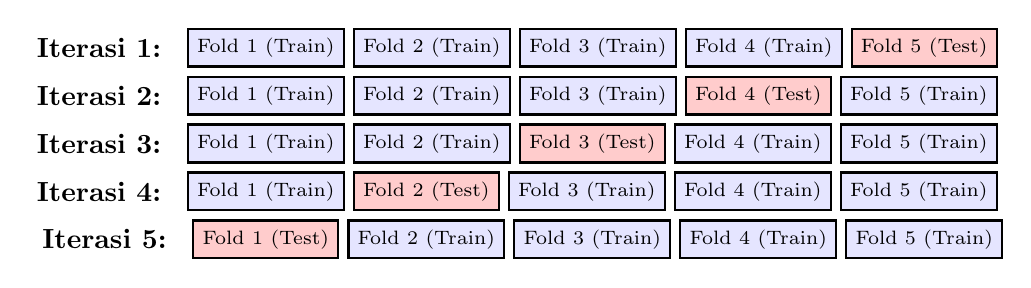
\begin{tikzpicture}[
        node distance=0.4cm,
        fold/.style={draw, thick, fill=blue!10, minimum width=1.6cm, minimum height=0.42cm, font=\scriptsize},
        test_fold/.style={draw, thick, fill=red!20, minimum width=1.6cm, minimum height=0.42cm, font=\scriptsize}
    ]
    % Iterasi 1
    \node[fold] (f1_1) {Fold 1 (Train)};
    \node[fold, right=0.1cm of f1_1] (f1_2) {Fold 2 (Train)};
    \node[fold, right=0.1cm of f1_2] (f1_3) {Fold 3 (Train)};
    \node[fold, right=0.1cm of f1_3] (f1_4) {Fold 4 (Train)};
    \node[test_fold, right=0.1cm of f1_4] (f1_5) {Fold 5 (Test)};
    \node[left=0.2cm of f1_1] {\textbf{Iterasi 1:}};
    
    % Iterasi 2
    \node[fold, below=0.1cm of f1_1] (f2_1) {Fold 1 (Train)};
    \node[fold, right=0.1cm of f2_1] (f2_2) {Fold 2 (Train)};
    \node[fold, right=0.1cm of f2_2] (f2_3) {Fold 3 (Train)};
    \node[test_fold, right=0.1cm of f2_3] (f2_4) {Fold 4 (Test)};
    \node[fold, right=0.1cm of f2_4] (f2_5) {Fold 5 (Train)};
    \node[left=0.2cm of f2_1] {\textbf{Iterasi 2:}};
    
    % Iterasi 3
    \node[fold, below=0.1cm of f2_1] (f3_1) {Fold 1 (Train)};
    \node[fold, right=0.1cm of f3_1] (f3_2) {Fold 2 (Train)};
    \node[test_fold, right=0.1cm of f3_2] (f3_3) {Fold 3 (Test)};
    \node[fold, right=0.1cm of f3_3] (f3_4) {Fold 4 (Train)};
    \node[fold, right=0.1cm of f3_4] (f3_5) {Fold 5 (Train)};
    \node[left=0.2cm of f3_1] {\textbf{Iterasi 3:}};

    % Iterasi 4
    \node[fold, below=0.1cm of f3_1] (f4_1) {Fold 1 (Train)};
    \node[test_fold, right=0.1cm of f4_1] (f4_2) {Fold 2 (Test)};
    \node[fold, right=0.1cm of f4_2] (f4_3) {Fold 3 (Train)};
    \node[fold, right=0.1cm of f4_3] (f4_4) {Fold 4 (Train)};
    \node[fold, right=0.1cm of f4_4] (f4_5) {Fold 5 (Train)};
    \node[left=0.2cm of f4_1] {\textbf{Iterasi 4:}};

    % Iterasi 5
    \node[test_fold, below=0.1cm of f4_1] (f5_1) {Fold 1 (Test)};
    \node[fold, right=0.1cm of f5_1] (f5_2) {Fold 2 (Train)};
    \node[fold, right=0.1cm of f5_2] (f5_3) {Fold 3 (Train)};
    \node[fold, right=0.1cm of f5_3] (f5_4) {Fold 4 (Train)};
    \node[fold, right=0.1cm of f5_4] (f5_5) {Fold 5 (Train)};
    \node[left=0.2cm of f5_1] {\textbf{Iterasi 5:}};
    
    \end{tikzpicture}
    \end{adjustbox}
  \end{figure}
  \begin{center}
    \fontsize{8pt}{10pt}\selectfont
    \textbf{Kebijakan Validasi Tanpa Kebocoran Data (Data Leakage-Free):}\\
    Pemisahan \textit{fold} dilakukan secara ketat pada \textbf{tingkat sampel tanah (24 lokasi geografi)}, bukan tingkat tembakan laser individual. Hal ini menjamin seluruh spektrum tembakan dari satu lokasi yang sama selalu dikelompokkan ke \textit{fold} yang sama guna mencegah bias optimasi.
  \end{center}
\end{frame}

% ==========================================
% Bagian D. PoC dan Penutup
% ==========================================
\section{PoC dan Penutup}

% Slide 27: Rencana Pengujian: Alokasi Sumber Daya & Jadwal Penelitian
\begin{frame}{Alokasi Sumber Daya \& Jadwal Penelitian}
  \begin{columns}[t]
    \begin{column}{0.45\textwidth}
      \small
      \textbf{1. Akuisisi Data Eksperimen}
      \fontsize{7.5pt}{9pt}\selectfont
      \begin{itemize}
        \item \textbf{Lokasi:} Laboratorium Gelombang dan Optik, Departemen Fisika, Fakultas Matematika dan Ilmu Pengetahuan Alam, Universitas Syiah Kuala (USK).
        \item \textbf{Tugas:} Preparasi sampel tanah vulkanik, penembakan laser, dan akuisisi spektrum emisi LIBS.
      \end{itemize}

      \vspace{0.4em}
      \small
      \textbf{2. Simulasi \& Pelatihan Model}
      \fontsize{7.5pt}{9pt}\selectfont
      \begin{itemize}
        \item \textbf{Infrastruktur:} Kluster GPU Mahameru HPC BRIN.
        \item \textbf{Tugas:} Pembangkitan spektrum sintetis (100k data) dan pelatihan model CNN-Transformer (Pre-training \& GRL).
      \end{itemize}
    \end{column}

    \begin{column}{0.53\textwidth}
      \centering
      \small\textbf{Jadwal Pelaksanaan Penelitian}
      \vspace{0.3em}
      
      \renewcommand{\arraystretch}{1.25}
      \begin{adjustbox}{max width=\textwidth}
        \begin{tabular}{|p{3.5cm}|*{12}{c|}}
          \hline
          \textbf{Nama Kegiatan} & \multicolumn{12}{c|}{\textbf{Tahun Pertama Bulan ke-}} \\
          \cline{2-13}
          & 1 & 2 & 3 & 4 & 5 & 6 & 7 & 8 & 9 & 10 & 11 & 12 \\
          \hline
          1. Pembangkitan spektrum sintetis & $\checkmark$ & $\checkmark$ & $\checkmark$ & $\checkmark$ & $\checkmark$ & & & & & & & \\
          \hline
          2. Preparasi sampel \& pengukuran LIBS (Lab Optik USK) & & & $\checkmark$ & $\checkmark$ & $\checkmark$ & $\checkmark$ & & & & & & \\
          \hline
          3. Desain, \textit{pre-training} \& \textit{fine-tuning} (HPC BRIN) & & & & $\checkmark$ & $\checkmark$ & $\checkmark$ & $\checkmark$ & $\checkmark$ & $\checkmark$ & $\checkmark$ & & \\
          \hline
          4. Analisis performa \& penulisan tesis / manuskrip & & & & & & $\checkmark$ & $\checkmark$ & $\checkmark$ & $\checkmark$ & $\checkmark$ & $\checkmark$ & $\checkmark$ \\
          \hline
        \end{tabular}
      \end{adjustbox}
    \end{column}
  \end{columns}
\end{frame}

% Slide 29: Kesimpulan \& Kontribusi Penelitian
\begin{frame}{Kesimpulan \& Kontribusi Penelitian}
  \begin{figure}[H]
    \centering
    \resizebox{!}{0.48\textheight}{
    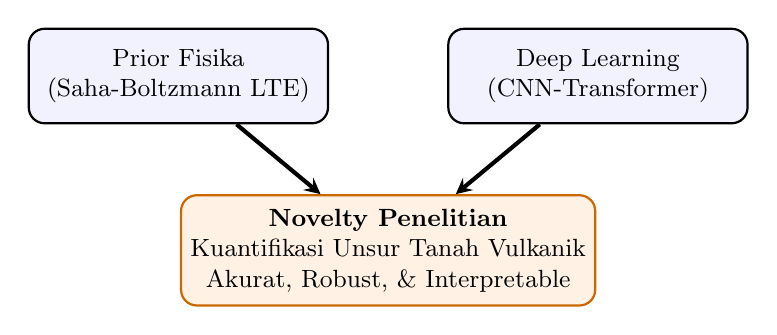
\begin{tikzpicture}[
        scale=0.9,
        font=\small,
        concept/.style={draw, thick, fill=blue!5, rounded corners=2mm, align=center, minimum width=3.8cm, minimum height=1.2cm},
        target/.style={draw=orange!80!black, thick, fill=orange!10, rounded corners=2mm, align=center, minimum width=4.2cm, minimum height=1.4cm},
        arrow/.style={-stealth, line width=1.5pt}
    ]
    % Nodes
    \node[concept] (phys) {Prior Fisika\\ \small (Saha-Boltzmann LTE)};
    \node[concept, right=1.5cm of phys] (dl) {Deep Learning\\ \small (CNN-Transformer)};
    \node[target, below=1.5cm of $(phys)!0.5!(dl)$] (novelty) {\textbf{Novelty Penelitian}\\ \small Kuantifikasi Unsur Tanah Vulkanik\\ \small Akurat, Robust, \& Interpretable};
    
    \draw[arrow] (phys) -- (novelty);
    \draw[arrow] (dl) -- (novelty);
    \end{tikzpicture}
    }
  \end{figure}
  \begin{center}
    \large\textcolor{uskGold}{\textbf{Terima Kasih atas Perhatian Anda}} \\[0.5em]
    {\normalsize Sesi Tanya Jawab \& Diskusi Dibuka}
  \end{center}
\end{frame}

\end{document}
